\begin{figure}
  \centering
  \begin{subfigure}[b]{0.6\textwidth}
    \centering
    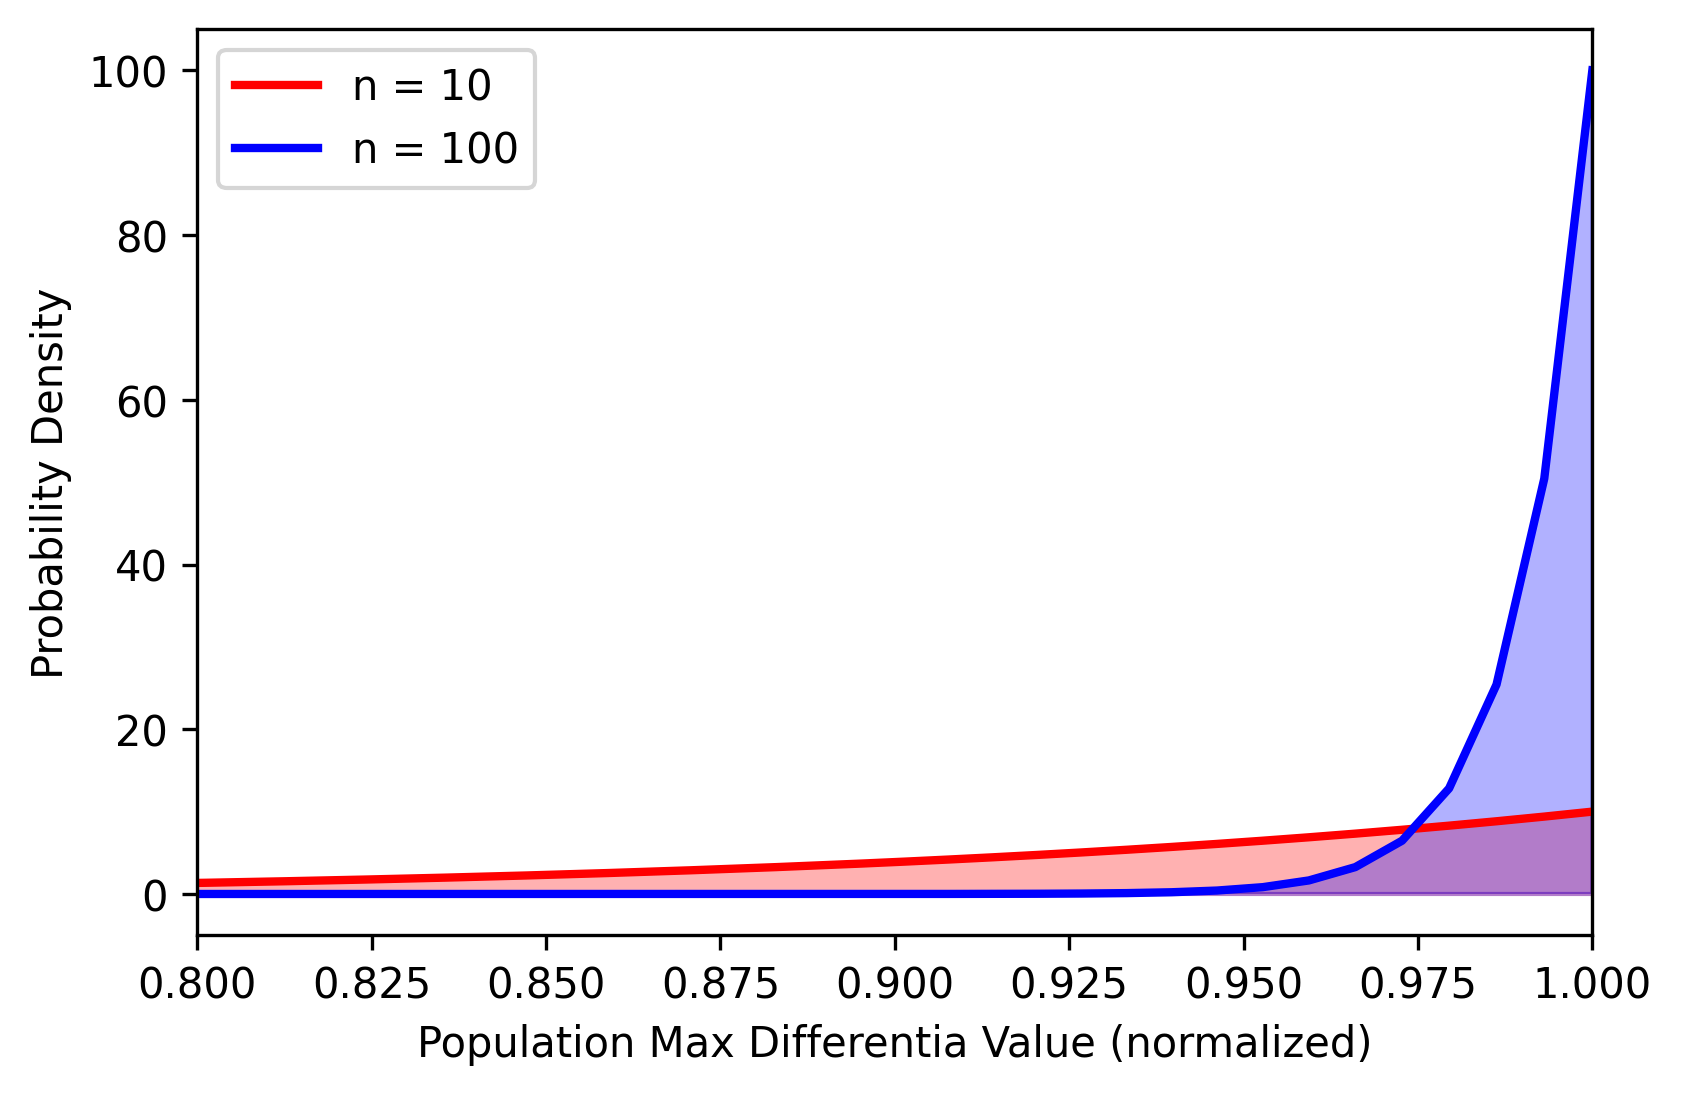
\includegraphics[width=\textwidth]{notebooks/notebooks/teeplots/viz=beta-pdf+ext=}
    % \caption{empty}
    % \label{fig:empty}
  \end{subfigure}%
  \begin{subfigure}[b]{0.4\textwidth}
    \centering
    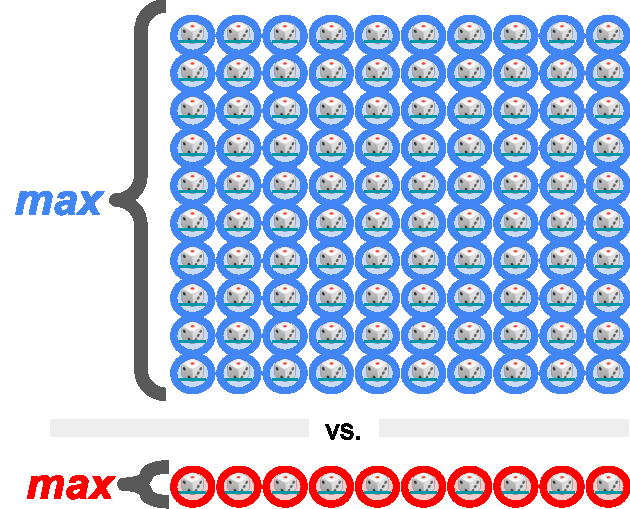
\includegraphics[width=\textwidth]{img/dice-pool}
    \vspace{3ex}
    % \caption{empty}
    % \label{fig:empty}
  \end{subfigure}
  \caption{
    Working principle of population size estimation.
    Increasing population size skews probability density function for population maximum value of generated fingerprints (referred to above as ``differentia'').
  }
  \label{fig:beta-explain}
\end{figure}
